% =====================================================================
%  PostLab 3 · Caracterización de diodos
%  Instrumentación Electrónica · Grado en Física · USAL · 2026/2027
%  Compilar:  latexmk -pdf main.tex
%  - img/*.jpg: fotos corregidas con scripts/corregir_fotos.py
%  - datos/*.dat: medidas recuperadas de Diodos_comparativa.pdf con
%    scripts/extraer_datos.py
% =====================================================================
\documentclass[10pt,a4paper]{article}
\usepackage{estilo}
\newcommand{\Vu}{V_u}
\colorlet{cBlancoM}{teal!70}

\begin{document}

% =====================================================================
%                              PORTADA
% =====================================================================
\thispagestyle{empty}
\noindent\begin{tikzpicture}[remember picture,overlay]
  \shade[top color=azulclaro!70,bottom color=white]
    ($(current page.north west)+(0,-0.35)$) rectangle
    ($(current page.north east)+(0,-6.0)$);
  \shade[left color=navy,right color=azulmed!45,middle color=azul!85]
    (current page.north west) rectangle ($(current page.north east)+(0,-0.35)$);
  \shade[left color=navy,right color=azulmed!45,middle color=azul!85]
    (current page.south west) rectangle ($(current page.south east)+(0,0.35)$);
\end{tikzpicture}\par
\vspace*{-0.4cm}
\noindent
\begin{tabularx}{\linewidth}{@{}l>{\centering\arraybackslash}Xr@{}}
  \raisebox{-.5\height}{
\includegraphics[height=1.0cm]{img/logo-usal.png}} &
  \begin{tabular}{@{}c@{}}
    {\color{navy}\large\textls[120]{\textsc{Universidad de Salamanca}}}\\[2pt]
    {\color{grisazul}\small\textls[100]{\textsc{Facultad de Ciencias\ \ $\cdot$\ \ Grado en Física}}}
  \end{tabular} &
  \raisebox{-.5\height}{
\includegraphics[height=0.95cm]{img/logo-ciencias.png}}
\end{tabularx}
\par\vspace{6pt}
\noindent{\color{grisclaro}\rule{\linewidth}{.6pt}}
\vspace{0.8cm}

\noindent{\color{azul}\large\textls[150]{\textsc{Instrumentación Electrónica\ \ $\cdot$\ \ PostLab 3}}}
\par\vspace{0.3cm}
\noindent{\fontsize{30}{36}\selectfont\bfseries\color{navy}Caracterización de diodos\par}
\vspace{6pt}
\noindent\tikz\shade[left color=navy,right color=white,middle color=azul]
  (0,0) rectangle (0.5\linewidth,2.6pt);
\par\vspace{0.35cm}
\noindent{\large\itshape\color{black!80}
Curvas $I_D(V_D)$ de un diodo pn, un diodo Zener y seis LED medidas con un
DAQ y un instrumento virtual en LabVIEW; tensiones umbral, tensión Zener y
su relación con el color de la luz emitida\par}
\vspace{0.55cm}

\noindent% Ilustración de la portada: diodos y LED sobre las curvas I-V medidas
\tikzset{
  pics/led/.style args={#1/#2/#3}{code={%
    % halo de luz (#3 = intensidad)
    \foreach \r/\o in {2.3/0.05,1.8/0.08,1.4/0.11,1.1/0.14}
      \fill[#2,opacity=#3*\o] (0,2.2) circle (\r);
    % patillas: ánodo (larga) y cátodo (corta)
    \fill[gray!60,draw=gray!30,line width=.2pt] (-0.42,-2.5) rectangle (-0.30,0);
    \fill[gray!60,draw=gray!30,line width=.2pt] (0.30,-2.0) rectangle (0.42,0);
    % electrodos internos: poste (ánodo) y yunque (cátodo)
    \fill[gray!55,opacity=.85] (-0.42,0) -- (-0.42,1.45) -- (-0.18,1.62) -- (-0.08,1.62)
      -- (-0.08,1.35) -- (-0.30,1.25) -- (-0.30,0) -- cycle;
    \fill[gray!55,opacity=.85] (-0.02,0.8) -- (-0.02,1.55) -- (0.08,1.55) -- (0.18,1.25)
      -- (0.48,1.25) -- (0.58,1.55) -- (0.72,1.55) -- (0.72,0.8) -- (0.42,0.8)
      -- (0.42,0) -- (0.30,0) -- (0.30,0.8) -- cycle;
    \fill[white,opacity=#3*.9] (0.33,1.33) circle (0.08);
    % cápsula de epoxi
    \shade[left color=#1!70!black,right color=#1!45!white,middle color=#1,opacity=.80]
      (-0.9,0.28) -- (-0.9,2.2) arc (180:0:0.9) -- (0.9,0.28) -- cycle;
    \fill[white,opacity=.40,rounded corners=2pt] (-0.70,0.50) rectangle (-0.52,2.15);
    \fill[white,opacity=.25] (-0.35,2.75) circle (0.18);
    \shade[top color=#1!75!white,bottom color=#1!60!black,opacity=.95]
      (-1.05,0) rectangle (0.95,0.28);
    \draw[#1!40!black,line width=.35pt] (-0.9,0.28) -- (-0.9,2.2) arc (180:0:0.9) -- (0.9,0.28);
  }},
  pics/axial/.style args={#1/#2/#3}{code={%
    \draw[gray!55,line width=1.1pt] (-2.1,0) -- (2.1,0);
    \shade[top color=#1!60!white,bottom color=#1!70!black,middle color=#1,rounded corners=3pt]
      (-0.95,-0.34) rectangle (0.95,0.34);
    \fill[white,opacity=.25,rounded corners=2pt] (-0.85,0.12) rectangle (0.85,0.26);
    \fill[#2] (#3,-0.34) rectangle ($(#3,0.34)+(0.2,0)$);
  }},
}
\colorlet{dpn}{black!80}\colorlet{dzener}{orange!75!red}
\colorlet{ledIR}{violet!45!gray}\colorlet{ledB}{white!80!gray}
\begin{tikzpicture}
  \def\W{16.9}\def\H{6.3}
  \begin{scope}
    \clip[rounded corners=6pt] (0,0) rectangle (\W,\H);
    \shade[left color=navy!95!black,right color=azul!75!navy] (0,0) rectangle (\W,\H);
    \fill[white,opacity=.04] (\W*0.55,\H) circle (5.5);
    % curvas I-V medidas, en segundo plano
    \begin{axis}[at={(0,0)},anchor=south west,scale only axis,width=\W cm,height=\H cm,
      hide axis,xmin=-2.7,xmax=3.0,ymin=-3.1,ymax=4.9,clip=false]
      \draw[white,opacity=.18] (axis cs:-2.7,0) -- (axis cs:3,0);
      \draw[white,opacity=.18] (axis cs:0,-3.1) -- (axis cs:0,4.9);
      \foreach \fic/\col in {pn/gray!40,zener/cZener,ir/violet!70,rojo/cRojo,
          amarillo/Gold,verde/cVerde,azul/cAzul!70!cyan,blanco/cyan!40}{
        \edef\temp{\noexpand\addplot[\col,line width=1.3pt,opacity=.38]
          table[x=VD,y=ID]{datos/\fic.dat};}
        \temp}
    \end{axis}
  \end{scope}
  \draw[white,opacity=.25,rounded corners=6pt] (0,0) rectangle (\W,\H);
  % ---------- diodos de unión
  \pic[scale=0.62] at (2.65,4.6) {axial=dpn/gray!15/0.42};
  \node[white,font=\sffamily\scriptsize,align=center] at (2.65,4.0)
    {\textbf{Diodo pn}\ \ $V_u=\SI{0.60}{V}$};
  \pic[scale=0.62] at (2.65,2.85) {axial=dzener/black!85/0.42};
  \node[white,font=\sffamily\scriptsize,align=center] at (2.65,2.25)
    {\textbf{Zener}\ \ $V_u=\SI{0.72}{V}$\ \ $|V_Z|=\SI{1.85}{V}$};
  % símbolos
  \begin{scope}[shift={(0.55,0.75)},scale=0.62,transform shape,color=white]
    \draw[white] (0,0) to[D*,color=white] (1.9,0);
    \draw[white] (2.5,0) to[zD*,color=white] (4.4,0);
    \draw[white] (5.0,0) to[leD*,color=white] (6.9,0);
  \end{scope}
  % ---------- LED
  \foreach \x/\cb/\cg/\i/\n/\v in {
      6.2/ledIR/violet/0.55/IR/1.10,
      7.9/cRojo/red/1/Rojo/1.63,
      9.6/Gold/yellow/1/Amarillo/1.77,
      11.3/cVerde/green/1/Verde/1.81,
      13.0/cAzul/cyan!60!blue/1/Azul/2.51,
      14.7/ledB/white/1/Blanco/2.58}{
    \begin{scope}
      \clip[rounded corners=6pt] (0,0) rectangle (\W,\H);
      \pic[scale=0.78] at (\x,2.0) {led=\cb/\cg/\i};
    \end{scope}
    \node[white,font=\sffamily\scriptsize\bfseries] at (\x,5.18) {\n};
    \node[white,opacity=.9,font=\sffamily\tiny] at (\x,4.86) {$V_u=\SI{\v}{V}$};
  }
  \draw[-{Stealth[length=5pt]},white,opacity=.7] (6.4,5.75) -- (14.7,5.75)
    node[midway,above=-1pt,font=\sffamily\tiny,opacity=1]{menor $\lambda$\ \ $\Rightarrow$\ \ mayor tensión umbral};
\end{tikzpicture}

\vspace{0.55cm}

\noindent
\begin{minipage}[t]{0.62\linewidth}
  {\color{azul}\small\textls[120]{\textsc{Autores}}}\\[3pt]
  {\large Miguel Martín Cortés}\ \ {\small\color{grisazul}70974284X}\\[1pt]
  {\large Álvaro Montero Mateos}\ \ {\small\color{grisazul}71096223A}\\[1pt]
  {\large Daniel Martín Guerrero}\ \ {\small\color{grisazul}71063727Y}
\end{minipage}%
\begin{minipage}[t]{0.38\linewidth}
  {\color{azul}\small\textls[120]{\textsc{Grupo}}}\\[3pt]
  {\large C.2}\\[6pt]
  {\color{azul}\small\textls[120]{\textsc{Asignatura}}}\\[3pt]
  {\large Instrumentación Electrónica}\\
  {\small\color{grisazul}Grado en Física, 2.º curso}
\end{minipage}
\par\vspace{0.55cm}

\noindent
\begin{tcolorbox}[enhanced,sharp corners,boxrule=0pt,frame hidden,
  borderline west={2.2pt}{0pt}{navy},
  interior style={left color=azulclaro,right color=white},
  left=9pt,right=8pt,top=6pt,bottom=6pt,width=\linewidth]
  {\color{navy}\textls[120]{\textsc{Resumen}}}\par\vspace{3pt}
  \small
  Hemos construido en LabVIEW un trazador de curvas: el DAQ barre la tensión
  aplicada a un circuito $R$--diodo de $-5$ a $\SI{5}{V}$ en 150 pasos, mide
  la tensión del diodo y calcula su corriente. Con él medimos la característica
  de ocho diodos y, ajustando por mínimos cuadrados el tramo de conducción,
  obtenemos las tensiones umbral, de $\SI{0.60}{V}$ (pn) a $\SI{2.58}{V}$
  (LED blanco), y una tensión Zener de $\SI{-1.85}{V}$. En los LED, el umbral
  crece con la energía del fotón emitido con una pendiente de $1{,}04$, muy
  cerca del valor ideal $eV_u\simeq hc/\lambda$.
\end{tcolorbox}
\par\vspace{8pt}{\color{grisclaro}\hrule height .5pt}\vspace{8pt}
\noindent\hfill
$I_D=\dfrac{V_{\text{in}}-V_D}{R}$\hfill
$I_D=a+b\,V_D\ \Rightarrow\ V_u=-\dfrac{a}{b}$\hfill
$eV_u\simeq E_g\simeq\dfrac{hc}{\lambda}$\hfill\null
\par\vspace{8pt}{\color{grisclaro}\hrule height .5pt}

\vfill
\begin{center}
  {\color{grisazul}\textls[120]{\textsc{Salamanca, curso académico 2026/2027}}}
\end{center}
\newpage

% =====================================================================
\section{Introducción}
% =====================================================================

\noindent
\begin{minipage}[c]{0.50\linewidth}
  El objetivo de esta práctica es caracterizar una serie de diodos y determinar sus tensiones umbral. En caso del diodo Zener, determinar a su vez la tensión Zener.
  \par\vspace{0.3cm}
  Para la realización se hizo uso de una tarjeta de adquisición de datos o DAQ, cables, una resistencia, diodos (p-n, Zener, rojo, verde, azul, amarillo, blanco e infrarrojo) y un ordenador con el programa de intrumentación virtual LabView.El esquema del montaje se muestra a continuación:
\end{minipage}\hfill
\begin{minipage}[c]{0.47\linewidth}\centering
  \begin{tikzpicture}[scale=0.67,transform shape]
    \node[inner sep=0] (a) at (0,0) {% Circuito de caracterización R-LED con el DAQ
\begin{circuitikz}[font=\small,
  term/.style={-{Straight Barb[length=4pt]Straight Barb[length=4pt]},thick}]
  \draw (2,5) to[R,l_=$R$,i>^=$\ID$] (2,2.2) coordinate (n);
  \draw (n) to[leD*,l_=LED] (2,0) coordinate (g);
  \draw[term] (2,5) -- (0.3,5) node[left,cRojo!85!black,font=\bfseries]{AO-0};
  \draw[term] (n) -- (3.8,2.2) node[right,cAzul!85!black,font=\bfseries]{AI-1};
  \draw[term] (g) -- (3.8,0) node[right,font=\bfseries]{GND};
  \draw (g) -- (2,-0.3) node[ground]{};
  \fill (n) circle (1.8pt) (g) circle (1.8pt);
  \node[above left,azul,font=\scriptsize] at (2.05,1.7) {A};
  \node[below left,azul,font=\scriptsize] at (2.05,0.55) {K};
  % tensiones
  \draw[-{Stealth[length=6pt]},rojoaviso,thick] (0.6,0.1) -- node[left]{$\Vin$} (0.6,4.6);
  \draw[-{Stealth[length=6pt]},rojoaviso,thick] (3.3,0.1) -- node[right]{$\VD$} (3.3,1.95);
\end{circuitikz}
};
    \node[inner sep=0,anchor=west] at ($(a.east)+(0.3,0)$) {% Montaje en la protoboard (vista superior esquemática)
\begin{tikzpicture}[font=\scriptsize,
  cable/.style={line width=1.7pt,line cap=round,rounded corners=4pt}]
  \def\p{0.38}
  % coordenada del orificio (columna, fila) con filas a=0 ... e=4, f=6 ... j=10
  \newcommand{\hole}[2]{({#1*\p},{-#2*\p})}
  % placa
  \fill[gray!10,draw=gray!45,rounded corners=3pt] (0.05,1.25) rectangle ({17*\p-0.05},{-11*\p});
  \fill[gray!22] (0.15,{-4.75*\p}) rectangle ({17*\p-0.15},{-5.25*\p});
  % raíles de alimentación
  \draw[rojoaviso!80,line width=.7pt] (0.25,1.05) -- ({17*\p-0.25},1.05);
  \draw[cAzul!80,line width=.7pt] (0.25,0.35) -- ({17*\p-0.25},0.35);
  \foreach \c in {1,...,16}{
    \fill[gray!55] ({\c*\p-0.055},{0.85-0.055}) rectangle ++(0.11,0.11);
    \fill[gray!55] ({\c*\p-0.055},{0.55-0.055}) rectangle ++(0.11,0.11);}
  % orificios
  \foreach \c in {1,...,16}{
    \foreach \r in {0,...,4,6,7,8,9,10}
      \fill[gray!55] ({\c*\p-0.055},{-\r*\p-0.055}) rectangle ++(0.11,0.11);}
  \foreach \c in {1,5,10,15} \node[gray!70] at ({\c*\p},{0.13}) {\c};
  \foreach \r/\l in {0/a,4/e,6/f,10/j} \node[gray!70] at (0.13,{-\r*\p}) {\l};
  % tiras conectadas (columnas 3, 8 y 10, filas a-e)
  \foreach \c/\col in {3/cRojo,8/cAzul,10/black}
    \draw[\col!45,line width=3.2pt,opacity=.35,line cap=round] \hole{\c}{0} -- \hole{\c}{4};
  % resistencia 1 kOhm entre columnas 3 y 8 (fila b)
  \draw[gray!60!black,line width=.8pt] \hole{3}{1} -- \hole{8}{1};
  \fill[draw=brown!60!black,fill={rgb,255:red,227;green,201;blue,154},rounded corners=2.5pt]
     ({4.25*\p},{-\p-0.14}) rectangle ({6.75*\p},{-\p+0.14});
  \foreach \x/\c in {4.7/brown!70!black,5.15/black,5.6/red!85!black,6.3/Goldenrod}
     \fill[\c] ({\x*\p-0.04},{-\p-0.14}) rectangle ({\x*\p+0.04},{-\p+0.14});
  \node[above,font=\scriptsize\bfseries,brown!60!black] at ({5.5*\p},{-\p+0.12}) {$R$};
  % LED: ánodo columna 8, cátodo columna 10 (fila e)
  \coordinate (L) at ({9*\p},{-7.2*\p});
  \draw[gray!60!black,line width=.8pt] \hole{8}{4} -- ($(L)+(-0.12,0.1)$);
  \draw[gray!60!black,line width=.8pt] \hole{10}{4} -- ($(L)+(0.12,0.1)$);
  \begin{scope}
    \clip ($(L)+(-0.5,-0.5)$) rectangle ($(L)+(0.33,0.5)$);
    \shade[inner color=cRojo!40,outer color=cRojo!90!black] (L) circle (0.4);
  \end{scope}
  \draw[cRojo!60!black] ($(L)+(0.33,-0.226)$) -- ($(L)+(0.33,0.226)$);
  \fill[white,opacity=.6] ($(L)+(-0.13,0.12)$) circle (0.07);
  \node[azul,font=\scriptsize\bfseries] at ($(L)+(-0.62,0.0)$) {$+$};
  \node[azul,font=\scriptsize\bfseries] at ($(L)+(0.6,0.0)$) {$-$};
  % cables
  \draw[cable,rojoaviso] ({2.2*\p},2.0) -- ({2.2*\p},1.55) -- \hole{3}{0};
  \draw[cable,cAzul] ({8*\p},2.0) -- \hole{8}{0};
  \draw[cable,black!85] ({12.5*\p},2.0) -- ({12.5*\p},1.55) -- \hole{10}{0};
  \foreach \c in {3,8,10} \fill[black] ({\c*\p-0.06},{-0.06}) rectangle ++(0.12,0.12);
  \node[above,rojoaviso,font=\small\bfseries] at ({2.2*\p},2.0) {AO-0};
  \node[above,cAzul,font=\small\bfseries] at ({8*\p},2.0) {AI-1};
  \node[above,black!85,font=\small\bfseries] at ({12.5*\p},2.0) {GND};
\end{tikzpicture}
};
  \end{tikzpicture}
  \captionof{figure}{Montaje del circuito para la caracterización de los diodos \cite{guion_diodos}.}
  \label{fig:guiondiodos}
\end{minipage}

% =====================================================================
\section{El instrumento virtual en LabVIEW}
% =====================================================================

El programa funciona como un trazador de curvas \emph{cuasiestático}: impone un
valor de $V_{\text{in}}$, espera a que el circuito se estabilice, mide $V_D$,
calcula $I_D$ y pasa al siguiente valor. Cada punto $(V_D,I_D)$ es por tanto un
estado estacionario.

\subsection{Panel frontal}

\begin{figure}[htbp]
  \centering
  % Foto corregida del panel frontal con anotaciones
\begin{tikzpicture}[
  caja/.style={draw=#1,fill=white,fill opacity=.93,text opacity=1,rounded corners=1.5pt,
    font=\sffamily\scriptsize,inner sep=2.5pt,align=left,line width=.6pt},
  caja/.default=azul,
  flecha/.style={-{Stealth[length=4.5pt]},#1,line width=.8pt},
  flecha/.default=azul,
  num/.style={circle,fill=#1,text=white,font=\sffamily\bfseries\tiny,inner sep=0pt,
    minimum size=10pt,draw=white,line width=.5pt},
  num/.default=navy]
  \node[inner sep=0,anchor=south west] (img) at (0,0)
    {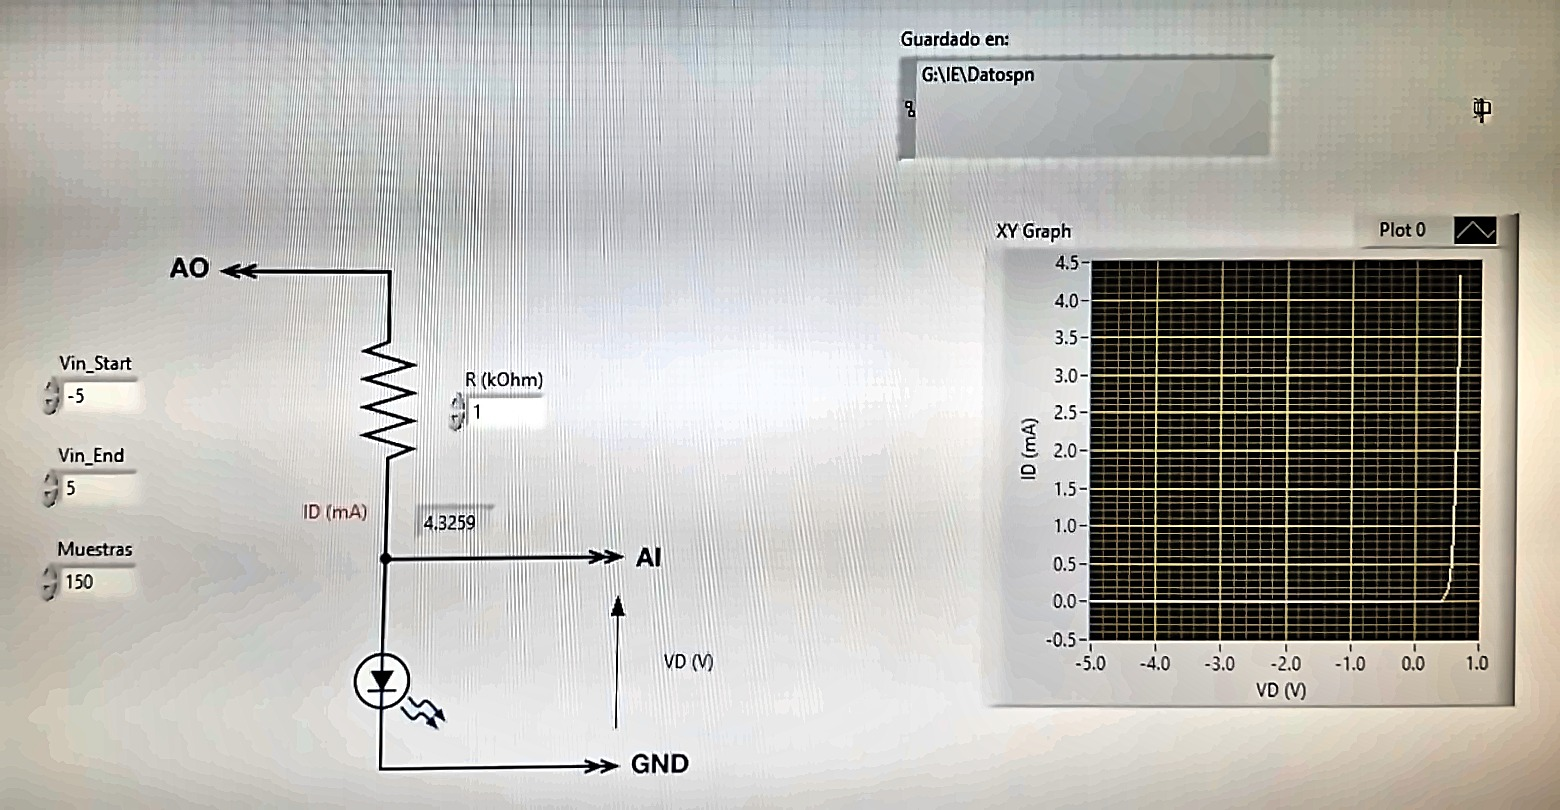
\includegraphics[width=\linewidth]{img/panel_frontal.jpg}};
  \begin{scope}[x={(img.south east)},y={(img.north west)}]
    % controles de la rampa
    \node[caja=ambar,anchor=west] (c) at (0.105,0.16)
      {\textbf{\textcolor{ambar}{\ding{172}} Controles numéricos (DBL)}\\
       rampa: $V_{\text{start}}=-5$\,V, $V_{\text{end}}=5$\,V,\\ 150 muestras};
    \draw[flecha=ambar] (c.north west) ++(0.012,0) -- (0.075,0.50);
    \draw[flecha=ambar] (c.north west) ++(0.022,0) -- (0.075,0.39);
    \draw[flecha=ambar] (c.west) -- (0.075,0.28);
    % R
    \node[caja=ambar,anchor=west] (r) at (0.36,0.62)
      {\textbf{\textcolor{ambar}{\ding{173}} Control $R$ (k$\Omega$)}\\ valor de la resistencia: 1};
    \draw[flecha=ambar] (r.west) -- (0.345,0.52);
    % indicador I_D
    \node[caja=cVerde,anchor=west] (i) at (0.455,0.43)
      {\textbf{\textcolor{cVerde}{\ding{174}} Indicador $I_D$ (mA)}\\ último valor: 4,326 mA\\ (con $V_{\text{in}}=5$\,V)};
    \draw[flecha=cVerde] (i.west) -- (0.335,0.37);
    % imagen del circuito
    \node[caja,anchor=north west] (img2) at (0.18,0.985)
      {\textbf{\textcolor{azul}{\ding{175}} Imagen importada (LED\_cir.png)}\\
       AO-0 impone $V_{\text{in}}$ sobre $R$ + diodo; AI-1 lee $V_D$;\\ GND es la masa común};
    \draw[flecha] (img2.south west) ++(0.03,0) -- (0.115,0.69);
    \draw[flecha] (img2.south) ++(0.02,0) -- (0.39,0.33);
    % ruta del fichero
    \node[caja=navy,anchor=east] (p) at (0.585,0.875)
      {\textbf{\textcolor{navy}{\ding{176}} Control de ruta}\\ fichero de salida (.txt)};
    \draw[flecha=navy] (p.east) -- (0.615,0.87);
    % gráfica XY
    \node[caja=cUV,anchor=east] (g) at (0.66,0.74)
      {\textbf{\textcolor{cUV}{\ding{177}} XY Graph}\\ eje $Y$: $I_D$ (mA)\\ eje $X$: $V_D$ (V)};
    \draw[flecha=cUV] (g.east) -- (0.74,0.66);
    % rama directa
    \node[caja=cUV,anchor=east] (k) at (0.905,0.56)
      {rama directa:\\ conduce a partir\\ de $V_u\approx0{,}6$\,V};
    \draw[flecha=cUV] (k.south east) ++(-0.005,0) -- (0.925,0.36);
    \node[caja=cUV,anchor=west] (corte) at (0.715,0.22)
      {corte: $I_D\simeq0$};
    \draw[flecha=cUV] (corte.north) -- (0.78,0.30);
  \end{scope}
\end{tikzpicture}

  \caption{Panel frontal del instrumento (foto de la pantalla con la
  perspectiva corregida), tras medir el diodo pn.}
  \label{fig:panel}
\end{figure}

El panel frontal (\cref{fig:panel}) es la interfaz con el usuario. En LabVIEW
se distingue entre \emph{controles}, que son entradas que el usuario fija antes
de ejecutar, e \emph{indicadores}, que son salidas que el programa escribe:

\begin{itemize}[leftmargin=1.2em]
  \item \textbf{\textcolor{ambar}{\ding{172}}\,\ding{173} Controles numéricos.}
    \ttt{Vin\_Start} y \ttt{Vin\_End} fijan los extremos de la rampa, de $-5$
    a $\SI{5}{V}$, que es el rango de la salida del DAQ. \ttt{Muestras} fija el
    número de puntos (150, un paso de $\approx\SI{67}{mV}$). \ttt{R (kOhm)} es
    el valor de la resistencia y solo interviene en el cálculo de $I_D$.
  \item \textbf{\textcolor{cVerde}{\ding{174}} Indicador \ttt{ID (mA)}.}
    Muestra la corriente de la iteración en curso. Al terminar queda el
    último valor, $\SI{4.326}{mA}$, que corresponde a
    $V_{\text{in}}=\SI{5}{V}$ y coincide con el máximo de la curva del diodo pn.
  \item \textbf{\textcolor{azul}{\ding{175}} Imagen del circuito}
    (\ttt{LED\_cir.png}). Es solo decorativa, pero recuerda el cableado: AO-0
    al extremo libre de $R$, AI-1 al nudo $R$--ánodo y el cátodo a GND.
  \item \textbf{\textcolor{navy}{\ding{176}} Control de ruta} \ttt{Guardado en}.
    Indica el fichero de texto donde se escriben los datos.
  \item \textbf{\textcolor{cUV}{\ding{177}} \ttt{XY Graph}.} Representa $I_D$
    (mA, eje vertical) frente a $V_D$ (V, eje horizontal) a medida que se
    mide. En la captura se ven el tramo de corte ($I_D\simeq0$ para $V_D<0$) y
    la subida brusca a partir de $\approx\SI{0.6}{V}$.
\end{itemize}

\subsection{Diagrama de bloques}

\begin{figure*}[htbp]
  \centering
  % Foto corregida del diagrama de bloques con zonas funcionales y elementos numerados
\begin{tikzpicture}[
  zona/.style={draw=#1,fill=#1,fill opacity=.07,draw opacity=.9,rounded corners=3pt,
    line width=.9pt,dashed},
  etq/.style={font=\sffamily\scriptsize\bfseries,text=#1,fill=white,draw=#1,
    rounded corners=1.5pt,inner sep=2pt,line width=.6pt},
  guia/.style={#1,line width=.7pt,-{Stealth[length=4pt]}},
  num/.style={circle,fill=navy,text=white,font=\sffamily\bfseries\fontsize{5.5}{6}\selectfont,
    inner sep=0pt,minimum size=9pt,draw=white,line width=.5pt}]
  \node[inner sep=0,anchor=south west] (img) at (0,0)
    {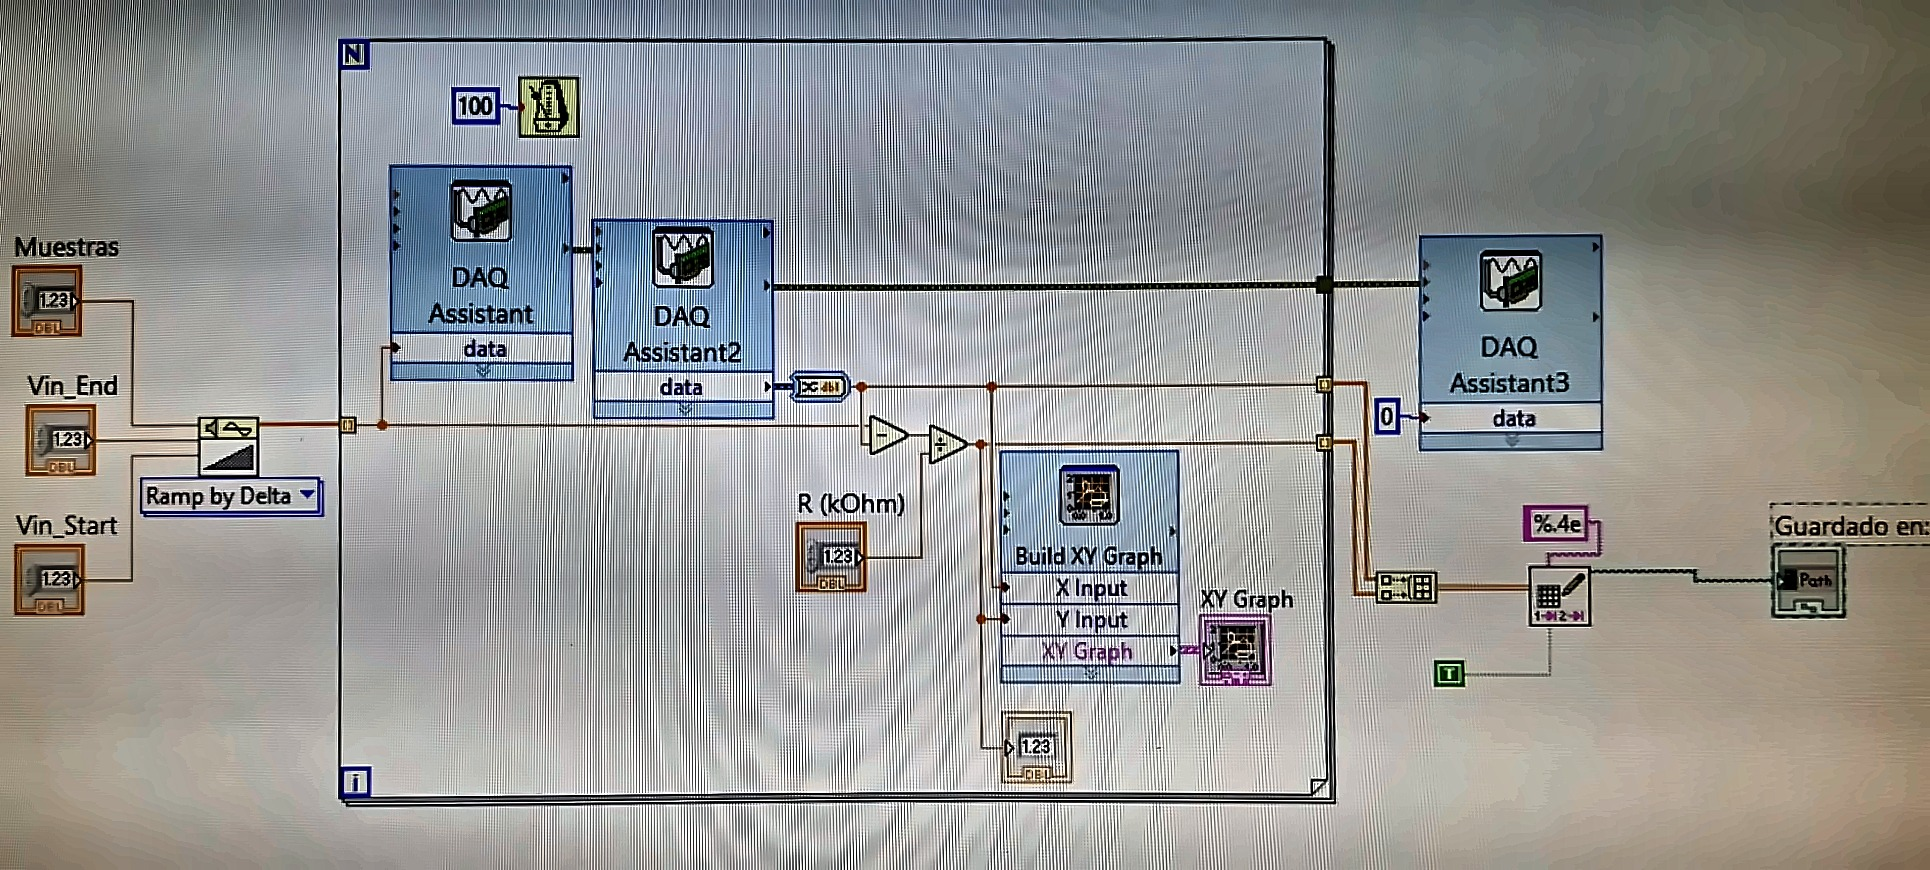
\includegraphics[width=\linewidth]{img/diagrama_bloques.jpg}};
  \begin{scope}[x={(img.south east)},y={(img.north west)}]
    % ---------------- zonas funcionales
    \draw[zona=ambar]     (0.004,0.275) rectangle (0.172,0.765);
    \draw[zona=grisazul]  (0.226,0.835) rectangle (0.322,0.93);
    \draw[zona=cRojo]     (0.218,0.545) rectangle (0.320,0.825);
    \draw[zona=cAzul]     (0.324,0.505) rectangle (0.418,0.785);
    \draw[zona=cVerde]    (0.412,0.305) rectangle (0.522,0.630);
    \draw[zona=cUV]       (0.524,0.085) rectangle (0.688,0.495);
    \draw[zona=cRojo]     (0.700,0.455) rectangle (0.842,0.745);
    \draw[zona=navy]      (0.700,0.175) rectangle (0.995,0.445);
    % ---------------- etiquetas de zona (fuera de la foto)
    \node[etq=ambar,anchor=south] (z1) at (0.085,1.035) {A\ \ Rampa de $V_{\text{in}}$};
    \draw[guia=ambar] (z1.south) -- (0.085,0.765);
    \node[etq=grisazul,anchor=south] (z2) at (0.255,1.035) {B\ \ Temporización};
    \draw[guia=grisazul] (z2.south) -- (0.27,0.93);
    \node[etq=cRojo,anchor=south] (z3) at (0.395,1.035) {C\ \ Salida AO-0};
    \draw[guia=cRojo] (z3.south) -- (0.30,0.825);
    \node[etq=cAzul,anchor=south] (z4) at (0.53,1.035) {D\ \ Adquisición AI-1};
    \draw[guia=cAzul] (z4.south) -- (0.40,0.785);
    \node[etq=cRojo,anchor=south] (z7) at (0.78,1.035) {G\ \ Reinicio AO-0 $=0$\,V};
    \draw[guia=cRojo] (z7.south) -- (0.78,0.745);
    \node[etq=grisazul,anchor=north] (zf) at (0.24,-0.04) {Bucle \ttt{For}: una medida por iteración};
    \draw[guia=grisazul] (zf.north) -- (0.24,0.07);
    \node[etq=cVerde,anchor=north] (z5) at (0.47,-0.04) {E\ \ Cálculo de $I_D$};
    \draw[guia=cVerde] (z5.north) -- (0.47,0.305);
    \node[etq=cUV,anchor=north] (z6) at (0.63,-0.04) {F\ \ Representación};
    \draw[guia=cUV] (z6.north) -- (0.63,0.085);
    \node[etq=navy,anchor=north] (z8) at (0.85,-0.04) {H\ \ Guardado en fichero};
    \draw[guia=navy] (z8.north) -- (0.85,0.175);
    % ---------------- elementos numerados
    \foreach \n/\x/\y in {1/0.072/0.700, 2/0.077/0.548, 3/0.072/0.385, 4/0.122/0.590,
        5/0.163/0.585, 6/0.214/0.940, 7/0.214/0.100, 8/0.233/0.812, 9/0.312/0.880,
        10/0.229/0.795, 11/0.333/0.757, 12/0.432/0.612, 13/0.455/0.445, 14/0.508/0.540,
        15/0.404/0.330, 16/0.536/0.472, 17/0.668/0.228, 18/0.566/0.118, 19/0.600/0.705,
        20/0.670/0.585, 21/0.748/0.722, 22/0.711/0.470, 23/0.722/0.385, 24/0.838/0.290,
        25/0.783/0.440, 26/0.776/0.228, 27/0.905/0.270}
      \node[num] at (\x,\y) {\n};
  \end{scope}
\end{tikzpicture}

  \caption{Diagrama de bloques del instrumento virtual (foto corregida).
  Las letras A--H marcan las etapas funcionales y los números los elementos
  que se describen en el texto y en la \cref{tab:simbolos}.}
  \label{fig:bloques}
\end{figure*}

La \cref{fig:bloques} muestra el código. Lo recorremos en el orden en que
fluyen los datos; los números remiten a la figura.

\paragraph{A. Rampa de tensiones.} Los tres controles \ttt{Muestras},
\ttt{Vin\_End} y \ttt{Vin\_Start} (1--3) entran en \ttt{Ramp Pattern} (4), que
genera un \emph{array} de 150 valores equiespaciados entre $-5$ y $\SI{5}{V}$.
El array (cable naranja grueso) entra en el bucle por un \emph{túnel con
auto-indexado} (5): en cada iteración el bucle toma el siguiente elemento.

\paragraph{Bucle \ttt{For}.} Repite el proceso una vez por cada valor de la
rampa. No hace falta cablear el terminal de cuenta \ttt{N} (6), porque el
auto-indexado fija el número de iteraciones al tamaño del array; \ttt{i} (7) es
el índice de la iteración en curso.

\paragraph{B. Temporización.} \ttt{Wait Until Next ms Multiple} (9) con la
constante entera \ttt{100} (8) sincroniza cada iteración con un múltiplo de
$\SI{100}{ms}$. Así se mide un punto cada $\SI{0.1}{s}$ (el barrido dura unos
$\SI{15}{s}$) y el circuito tiene tiempo de estabilizarse.

\paragraph{C--D. Salida y adquisición.} El primer \ttt{DAQ Assistant} (10)
está configurado como \emph{generación} de tensión en \ttt{ao0}, rango
$\pm\SI{5}{V}$ y modo \ttt{1 Sample (On Demand)}: en cada iteración escribe el
valor de $V_{\text{in}}$ que recibe en su entrada \ttt{data}. El segundo,
\ttt{DAQ Assistant2} (11), \emph{adquiere} una muestra de \ttt{ai1} en el mismo
modo~\cite{ni_daq}. Ambos van encadenados por el \emph{cable de error} (19), que obliga a
escribir antes de leer y detiene el programa si el DAQ da un fallo. La salida
del DAQ es de tipo \emph{datos dinámicos} y \ttt{Convert from Dynamic Data}
(12) la convierte en el número real $V_D$.

\paragraph{E. Cálculo de la corriente.} Con dos operadores aritméticos,
\ttt{Subtract} (13), que calcula $V_{\text{in}}-V_D$, y \ttt{Divide} (14), que
divide por el control \ttt{R (kOhm)} (15), se implementa la ley de Ohm en la
resistencia,
\begin{destacada}
  I_D\,(\si{mA})=\frac{V_{\text{in}}-V_D}{R\,(\si{k\ohm})}.
  \label{eq:ohm}
\end{destacada}
El resultado va al indicador \ttt{ID (mA)} (18).

\paragraph{F. Representación.} \ttt{Build XY Graph} (16) recibe $V_D$ en
\ttt{X Input} e $I_D$ en \ttt{Y Input} y alimenta el indicador \ttt{XY Graph}
(17). La opción \ttt{Clear data on each call} está desactivada para que los
puntos se acumulen y la curva se vaya dibujando.

\paragraph{G. Reinicio.} Al salir del bucle, \ttt{DAQ Assistant3} (21) escribe
la constante \ttt{0} (22) en AO-0 para no dejar el diodo polarizado. El cable de
error que sale del bucle (19) hace que esto ocurra solo cuando el barrido ha
terminado.

\paragraph{H. Guardado.} Los valores de $V_D$ e $I_D$ salen del bucle por
túneles con auto-indexado (20), que los acumulan en dos arrays de 150
elementos. \ttt{Build Array} (23) los une en una matriz 2D y \ttt{Write to
Spreadsheet File} (24) la escribe en el fichero de la ruta \ttt{Guardado en}
(27) con el formato \ttt{\%.4e} (25), es decir, notación exponencial con cuatro
decimales. La constante booleana \ttt{T} (26) activa \ttt{transpose}, de modo
que cada magnitud se guarda en una columna.

\begin{table}[htbp]
  \centering\footnotesize
  \caption{Simbología de LabVIEW que aparece en el diagrama.}
  \label{tab:simbolos}
  \renewcommand{\arraystretch}{1.12}
  \begin{tabularx}{\linewidth}{@{}l X l X@{}}
    \toprule
    \textbf{Símbolo} & \textbf{Significado} & \textbf{Símbolo} & \textbf{Significado}\\
    \midrule
    \tikz\draw[Orange!85!black,line width=1pt](0,0)--(0.7,0); & número real (DBL), un valor
      & \tikz\draw[Orange!85!black,line width=2.4pt,double=white,double distance=.5pt](0,0)--(0.7,0); & array de reales (rampa, columnas)\\
    \tikz\draw[blue!70!black,line width=1pt](0,0)--(0.7,0); & entero (constantes \ttt{100} y \ttt{0})
      & \tikz\draw[blue!40!black,line width=1.4pt,dash pattern=on 2pt off 1pt](0,0)--(0.7,0); & datos dinámicos (salidas del DAQ)\\
    \tikz\draw[Goldenrod!60!black,line width=1.6pt,dash pattern=on 3pt off 1pt](0,0)--(0.7,0); & cable de error: fija el orden de ejecución
      & \tikz\draw[magenta!80!black,line width=1pt](0,0)--(0.7,0); & cadena de texto (formato \ttt{\%.4e})\\
    \tikz\draw[green!50!black,line width=1pt](0,0)--(0.7,0); & booleano (constante \ttt{T})
      & \tikz\draw[teal,line width=1pt](0,0)--(0.7,0); & ruta de fichero (\ttt{Guardado en})\\
    borde grueso, $\triangleright$ a la derecha & control (entrada)
      & borde fino, $\triangleleft$ a la izquierda & indicador (salida)\\
    \raisebox{-1pt}{\tikz\draw[thick,fill=white](0,0) rectangle (0.18,0.18);} en el borde del bucle & túnel (con o sin auto-indexado)
      & \ttt{N}, \ttt{i} & n.º de iteraciones e índice del \ttt{For}\\
    \bottomrule
  \end{tabularx}
\end{table}

% =====================================================================
\section{Datos obtenidos}
% =====================================================================
Para poder tomar los datos se utilizó el programa mostrado en el apartado anterior y el circuito constituido por el diodo y una resistencia.
\par\vspace{0.2cm}
Las medidas tomadas para cada diodo se representaron gráficamente y se muestran a continuación:
\begin{figure}[htbp]
  \centering
  \begin{subfigure}[b]{0.53\linewidth}\centering
    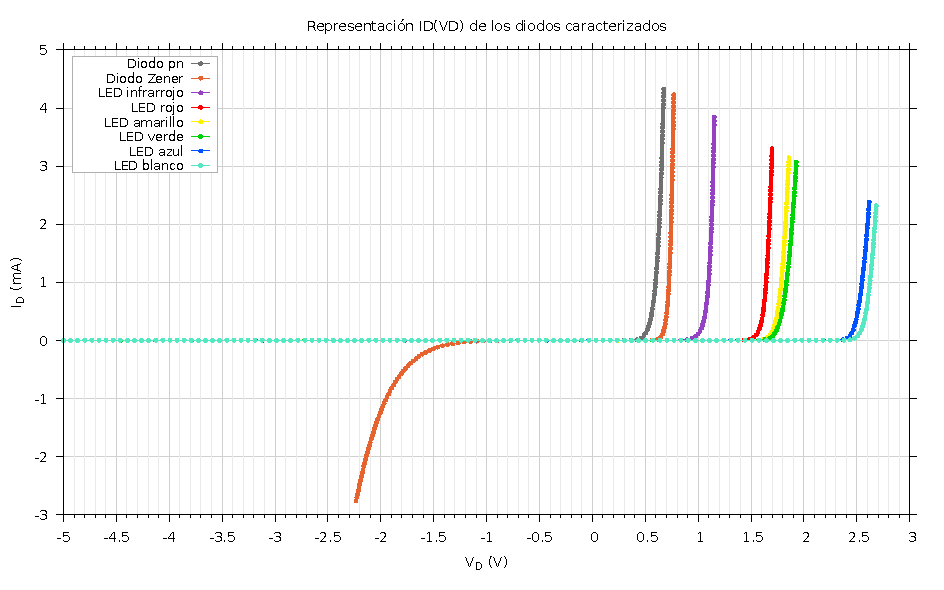
\includegraphics[width=\linewidth]{Diodos_comparativa.pdf}
    \caption{Vista general.}
  \end{subfigure}\hfill
  \begin{subfigure}[b]{0.44\linewidth}\centering
    % Ampliación de la rama directa con las rectas de ajuste (datos del grupo)
\colorlet{cBlancoM}{teal!70}
\pgfplotsset{
  serie/.style={#1,mark=*,mark size=.75pt,line width=.5pt},
  ajuste/.style={#1!70!black,dashed,line width=.7pt,forget plot},
}
\begin{tikzpicture}
\begin{axis}[width=\linewidth,height=5.0cm,grid=major,xlabel={$V_D$ (V)},
  ylabel={$I_D$ (mA)},xmin=0.35,xmax=2.98,ymin=-0.2,ymax=4.6]
  \foreach \fic/\col in {pn/cPN,zener/cZener,ir/cUV,rojo/cRojo,amarillo/cAmarillo,
      verde/cVerde,azul/cAzul,blanco/cBlancoM}{
    \edef\temp{\noexpand\addplot[serie=\col,forget plot] table[x=VD,y=ID]{datos/\fic.dat};}
    \temp}
  % rectas I = a + b V entre V_u y la corriente máxima
  \foreach \col/\a/\b/\vu/\imax in {
      cPN/-35.005/58.209/0.601/4.33, cZener/-67.097/92.632/0.724/4.25,
      cUV/-74.494/67.862/1.098/3.88, cRojo/-78.727/48.264/1.631/3.32,
      cAmarillo/-60.091/34.011/1.767/3.18, cVerde/-44.739/24.768/1.806/3.10,
      cAzul/-52.505/20.954/2.506/2.40, cBlancoM/-59.723/23.111/2.584/2.34}{
    \edef\temp{\noexpand\addplot[ajuste=\col,domain=\vu:(\imax-(\a))/(\b),samples=2]{\a+\b*x};
      \noexpand\fill[\col] (axis cs:\vu,0) circle (1.5pt);}
    \temp}
  \draw[black!50] (axis cs:0.35,0) -- (axis cs:2.98,0);
  \foreach \x/\y/\t in {0.67/4.42/pn,0.79/4.33/Zener,1.14/3.98/IR,1.68/3.42/rojo,
      1.83/3.28/amarillo,1.93/2.95/verde,2.62/1.75/blanco}{
    \edef\temp{\noexpand\node[font=\noexpand\tiny,anchor=south west,inner sep=1pt] at (axis cs:\x,\y) {\t};}
    \temp}
  \node[font=\tiny,anchor=south east,inner sep=1pt] at (axis cs:2.55,2.3) {azul};
\end{axis}
\end{tikzpicture}\\[2pt]
{\scriptsize\color{navy}$\bullet$\ $V_u=-a/b$\quad
 \tikz\draw[dashed,thick] (0,0.08)--(0.4,0.08);\ ajuste $I=a+bV$}

    \caption{Ampliación de la rama directa.}
  \end{subfigure}
  \caption{Comparativa de cada representación $I_D(V_D)$ para cada diodo. (b)
  Ampliación de la rama directa con las rectas de ajuste del
  \cref{sec:analisis}.}
  \label{fig:caida}
\end{figure}

% =====================================================================
\section{Análisis de datos}
\label{sec:analisis}
% =====================================================================
Observando los datos obtenidos, podemos determinar las tensiones umbral para cada diodo. Para esta empresa, hemos considerado que la mejor opción es aproximar aquellos puntos donde se observe una subida de intensidad considerable y aproximar todos esos puntos a una recta mediante una regresión lineal, para posteriormente buscar aquel valor de la tensión tal que hace cero la intensidad para cada una de las retas, determinando así la tensión umbral ($V_u$) para cada diodo.

\medskip
La recta de ajuste será:
\begin{destacada}
    I = a +bV
    \nonumber
\end{destacada}

\medskip
Hemos obtenido los siguientes coeficientes para cada diodo:

\noindent
\begin{minipage}[t]{0.48\linewidth}
  \vspace{0pt}\centering\footnotesize
  \renewcommand{\arraystretch}{1.12}
  \begin{tabular}{@{}l c c@{}}
    \toprule
    Diodo & a & b\\
    \midrule
    {\color{cPN}\rule{1.2ex}{1.2ex}}\ p-n & -35,005 & 58,209\\
    {\color{cZener}\rule{1.2ex}{1.2ex}}\ Zener & -67,097 & 92,632\\
    {\color{cZener}\rule{1.2ex}{1.2ex}}\ Zener ($V_{zener}$) & 12,939 & 7,007\\
    {\color{cBlancoM}\rule{1.2ex}{1.2ex}}\ Blanco & -59,723 & 23,111\\
    {\color{cAzul}\rule{1.2ex}{1.2ex}}\ Azul & -52,505 & 20,954\\
    {\color{cVerde}\rule{1.2ex}{1.2ex}}\ Verde & -44,739 & 24,768\\
    {\color{cAmarillo}\rule{1.2ex}{1.2ex}}\ Amarillo & -60,091 & 34,011\\
    {\color{cRojo}\rule{1.2ex}{1.2ex}}\ Rojo & -78,727 & 48,264\\
    {\color{cUV}\rule{1.2ex}{1.2ex}}\ Infrarrojo & -74,494 & 67,862\\
    \bottomrule
  \end{tabular}
  \captionof{table}{Coeficientes de ajuste para cada diodo, obtenidos mediante regresión lineal.}
  \label{tab:coef}
\end{minipage}\hfill
\begin{minipage}[t]{0.48\linewidth}
  \vspace{0pt}\centering\footnotesize
  \renewcommand{\arraystretch}{1.12}
  \begin{tabular}{@{}l c c@{}}
    \toprule
    Diodo & Intervalo $V_{u}$ [V] & Estimación $V_u$ [V]\\
    \midrule
    {\color{cPN}\rule{1.2ex}{1.2ex}}\ p-n & $0.5-0.7$ & 0,601\\
    {\color{cZener}\rule{1.2ex}{1.2ex}}\ Zener & $0.6-0.8$ & 0,724\\
    {\color{cBlancoM}\rule{1.2ex}{1.2ex}}\ Blanco & $2.4-2.6$ & 2,584\\
    {\color{cAzul}\rule{1.2ex}{1.2ex}}\ Azul & $2.4-2.5$ & 2,506\\
    {\color{cVerde}\rule{1.2ex}{1.2ex}}\ Verde & $1.8-1.9$ & 1,806\\
    {\color{cAmarillo}\rule{1.2ex}{1.2ex}}\ Amarillo & $1.6-1.8$ & 1,767\\
    {\color{cRojo}\rule{1.2ex}{1.2ex}}\ Rojo & $1.5-1.7$ & 1,631\\
    {\color{cUV}\rule{1.2ex}{1.2ex}}\ Infrarrojo & $0.9-1.1$ & 1,098\\
    \bottomrule
  \end{tabular}
  \captionof{table}{Tensiones umbrales para cada diodo.}
  \label{tab:umbrales}
\end{minipage}

\medskip
A partir de los coeficientes calculados en la tabla anterior obtenemos las tensiones umbral para cada uno de los diodos (\cref{tab:umbrales}).

\medskip
Destacar que por supuesto el valor exacto de los coeficientes varía en función de los puntos que utilicemos para realizar la regresión, sin embargo, concluimos que con el criterio utilizado para esta caracterización obtenemos resultados satisfactorios.

\medskip
Por otro lado, también podemos determinar la tensión Zener. En este caso hemos estimado un valor de: $V_z = -1.847\hspace{0.2cm}\text{V}$.

\medskip
Como comentario final, observamos que la tensión umbral de los LEDs aumenta con la frecuencia de la radiación electromagnética emitida y, por tanto, depende de su longitud de onda, es decir, de su color. A mayor frecuencia, mayor es la tensión que hay que aplicar para que el diodo sea capaz de conducir. Esto se debe a que la energía del fotón emitido es proporcional a su frecuencia, según el postulado de cuantización de Planck:
\begin{destacada}
    E = h\nu
\end{destacada}

\medskip
Por ende, se sigue que el LED azul deberá tener una tensión umbral mayor que cualquier otro, ya que es necesaria más energía para poder emitir luz de dicho color, lo cuál se ha demostrado con los resultados obtenidos.

\medskip
Asimismo, se observa que el LED blanco también posee una tensión umbral similar, esto es debido a que, en función de obtener luz blanca, se utiliza un LED azul con un recubrimiento de un material foto-luminiscente denominado fósforo, que da la sensación de blanco al ojo humano. Por ello, es esperable que las tensiones umbrales tanto del LED azul como del blanco sean similares.

\begin{figure}[htbp]
  \centering
  \begin{minipage}[c]{0.46\linewidth}\centering
    % Tensión umbral medida frente a la energía del fotón (lambda típica de catálogo)
\begin{tikzpicture}
\begin{axis}[width=\linewidth,height=5.3cm,xmin=1.15,xmax=2.85,ymin=0.9,ymax=2.9,
  xlabel={$E_{\text{ph}}=hc/\lambda$ (eV)},ylabel={$V_u$ (V)},grid=major,
  legend pos=north west,legend style={font=\tiny},legend cell align=left]
  \addplot[grisazul,thick,domain=1.15:2.85,samples=2]{x};
  \addlegendentry{$eV_u=E_{\text{ph}}$}
  \addplot[azul,dashed,thick,domain=1.15:2.85,samples=2]{1.0385*x-0.3605};
  \addlegendentry{ajuste: pendiente 1,04}
  \foreach \col/\e/\v/\t/\anc in {cUV/1.319/1.098/IR/north west,cRojo/1.984/1.631/rojo/north west,
      cAmarillo/2.101/1.767/amarillo/north west,cVerde/2.175/1.806/verde/south east,
      cAzul/2.638/2.506/azul/north west}{
    \edef\temp{\noexpand\addplot[only marks,mark=*,mark size=2.6pt,\col,draw=black!60,forget plot]
      coordinates {(\e,\v)};
      \noexpand\node[font=\noexpand\tiny,\col!80!black,anchor=\anc] at (axis cs:\e,\v) {\t};}
    \temp}
\end{axis}
\end{tikzpicture}

  \end{minipage}\hfill
  \begin{minipage}[c]{0.5\linewidth}
    \captionof{figure}{Complemento: $V_u$ de los LED de la \cref{tab:umbrales}
    frente a la energía del fotón $E=h\nu=hc/\lambda$, tomando longitudes de
    onda típicas de catálogo (IR 940, rojo 625, amarillo 590, verde 570, azul
    $\SI{470}{nm}$), no medidas. Los puntos se alinean sobre una recta de
    pendiente $1{,}04$, muy próxima a la relación ideal $eV_u=h\nu$.}
    \label{fig:energia}
  \end{minipage}
\end{figure}

{\small
\bibliographystyle{unsrt}
\bibliography{referencias}}

\end{document}
